%!TEX root = Humanoids2013.tex
\section{Problem Definition}

This paper considers novel soft-robotics actuation schemes which may enhance performance of mechanical systems in cyclic tasks, i.e.~reducing energy consumption, by exploiting the use of springs suitably placed on the system. For this reason, we study compliant mechanical systems which can be both fully actuated or underactuated. In the former case, there are as many actuators as Degrees of Freedom (DoF), whereas in the second one there are fewer control inputs than degrees of freedom~\cite{spong98}. 

Depending on how and where springs are placed on the system, the number of DoFs and the number of actuators, the dynamics of a mechanical system can assume particular forms as described in next subsections.

% An optimization method has been proposed to find the best actuation parameters for fully actuated and underactuated robots.  
% %The cost function and the index to minimize are based on the resulting motor torques and velocities.
% 
% Commonly underactuated mechanical systems are those mechanical systems that have fewer control inputs than degrees of freedom \cite{spong98}. In our work the underactuated mechanical systems denote the systems that have fewer actuator than degrees of freedom, whatever the nature of actuation is. As a consequence, the fully actuated systems are those systems that have as many actuators as degrees of freedom.
% We are particularly interested in studying compliant systems.

\subsection{Fully Actuated Mechanical Systems}
\label{sec:FullyActuatedSystems}

Let us first consider a fully actuated compliant mechanical system actuated by PEAs, e.g.~a spring between two links for a serial manipulator (see Fig.~\ref{fig:PEA}). For such a system, the number of DoFs remains equal to the number of actuators. Indicating by $q\in\Re^n$
the generalized coordinates representing the configuration of the system and by $\tau\in\Re^n$ the generalized torque provided by actuators, the dynamics can be written as
\begin{equation}
\label{eq:FullyActuated}
f(\ddot q,\dot q, q, t)=-K(q_e-q)+\tau\,,
\end{equation}
where $q_e\in\Re^n$ is the spring pre-load and $K\in\Re^{n\times n}$ is the stiffness matrix. The term $f(\ddot q,\dot q, q, t)$ includes inertia, coriolis, and gravity terms.
\begin{figure}[!t]
\centering
\subfigure[Example of robot actuated by PEA.]{\label{fig:PEA}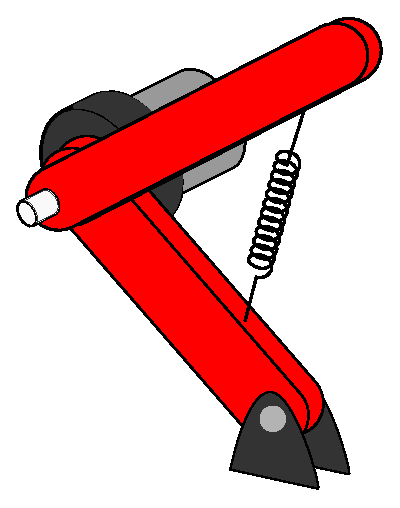
\includegraphics[width=0.25\columnwidth]{dwg/PEA}}
\quad
\subfigure[Example of robot actuated by SEA.]{\label{fig:SEA}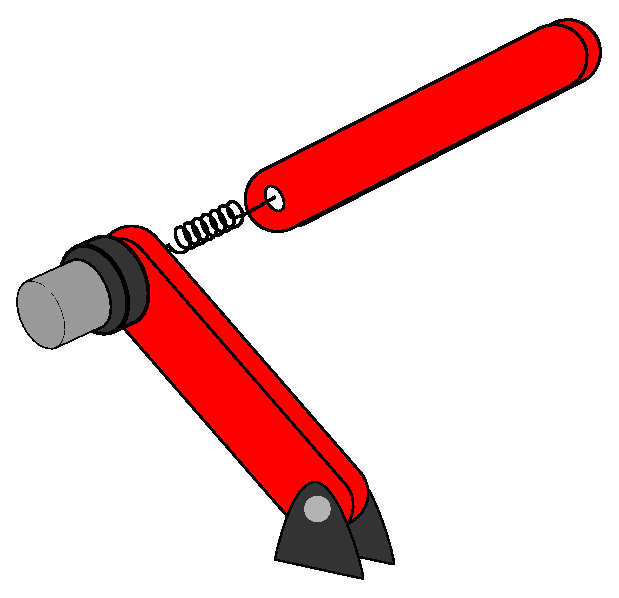
\includegraphics[width=0.4\columnwidth]{dwg/SEA}}
% 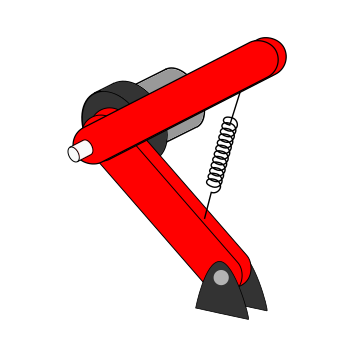
\includegraphics[width=0.4\columnwidth]{PEA}
\caption{Robot actuated by PEAs or SEAs.}
\label{fig:PEA_SEA}
\end{figure}

\subsection{Underactuated Mechanical Systems}
\label{sec:UnderActuatedSystems}

Consider now the case in which the mechanical system is actuated by SEAs (see Fig.~\ref{fig:SEA}), i.e.~the springs between the actuator and the load (e.g.~between the motor and the link for serial manipulators). Indicating by $\theta\in\Re^n$ the motor positions and by $J_m$ the inertia matrix of the motors, the dynamics can be written as
\begin{align}
\label{eq:actuated1_SEA}
f(\ddot{q}, \dot{q}, q, t) &= - K(q - \theta) \\
J_{m} \ddot{\theta} &= K(q - \theta) + \tau\,,
\label{eq:actuated2_SEA}
\end{align}
Notice that the use of SEAs instead of PEAs increases the number of DoFs which become $2n$. 

For particular mechanical systems there may be further DoFs which are not actuated, e.g.~the position and orientation of humanoids w.r.t. a fixed reference frame. Let $x\in\Re^m$ be those DoFs and assume the system is actuated by SEAs, the dynamics in this case can be written as 
\begin{align}
\label{eq:noact_SEAplus}
f_u(\ddot x, \dot x, x, \ddot{q}, \dot{q}, q, t) &= 0  \\
\label{eq:underact1_SEAplus}
f_a(\ddot x, \dot x, x, \ddot{q}, \dot{q}, q, t) &= - K(q - \theta)  \\
J_{m} \ddot{\theta} &= K(q - \theta)+\tau,
\label{eq:underact2_SEAplus}
\end{align}
where~\eqref{eq:noact_SEAplus} represents the non-actuated dynamics, whereas~\eqref{eq:underact1_SEAplus} and \eqref{eq:underact2_SEAplus} represent the underactuated dynamics.

Of course, if PEAs are used, the dynamics becomes
\begin{align}
\label{eq:noact_PEAplus}
f_u(\ddot x, \dot x, x, \ddot{q}, \dot{q}, q, t) &= 0  \\
\label{eq:underact_PEAplus}
f_a(\ddot x, \dot x, x, \ddot{q}, \dot{q}, q, t) &= - K(q_e - q)+\tau\,.
\end{align}
% \subsection{Fully Actuated Systems}
% 
% The general dynamics model of a n-DoF fully actuated system, using series elastic actuators can be written as 
% \begin{equation}
% f(\ddot{q}, \dot{q}, q, t)= - K(q - \theta)  
% \label{eq:actuated1}
% \end{equation}
% \begin{equation}
% J_{m} \ddot{\theta} - K(q - \theta) =  \tau,
% \label{eq:actuated2}
% \end{equation}
% where $f \in\Re^{n\times 1}$ is the dynamics expression of the system, which includes the inertia terms, the coriolis terms, and the gravity terms. 
% $q \in\Re^{n}$ is the vector of desired trajectories for each link, $\theta \in\Re^{n}$ is the vector of motor positions.
% $K \in\Re^{n\times n}$ is the elastic elements matrix, and $J_{m} \in\Re^{n \times n}$ is the motor's inertia matrix.
% $\tau \in \Re^{n}$ is the actuators torque.  
% 
% For n-DoF fully actuated systems with parallel elastic actuation, the dynamics model is
% \begin{equation}
% f(\ddot{q}, \dot{q}, q, t)= - K(q_e - q) + \tau \, ,  
% \label{eq:actuatedPEA}
% \end{equation}
% where $q_e \in \Re^{n}$ is the actuator pre-load.  

%%%%%%%%%

\subsection{Optimal Problem Formulation}

In order to quantify the performance of the mechanical system and hence to determine optimal joint stiffness $\hat K$ and/or pre-load $\hat q_e$ values as well as optimal joint trajectories $q(t)$, we will consider two different cost functionals:

\subsubsection{Squared-Power index}
Assuming that the motor spends energy if the mechanical power is positive or negative, the cost functional of the whole mechanical system is 
\begin{equation}
	J_1 = \sum_{j=1}^{n} \int_0^T(\tau_{j}(t)\dot{\theta_{j}}(t))^2dt\,,
\label{eq:J2}
\end{equation}
where $T$ represents the period of the cyclic task or its multiple. %energy spent by each actuator to accomplish the desired task: 
%\begin{equation}
%	J_1 = \sum_{j=1}^{m} \int_0^T{(\tau_{j}\dot{\theta_{j}}(t))dt}\, ,
%	\label{eq:J1}	
%\end{equation}

%This index serves if the actuators can store energy when the mechanical power is negative. Nevertheless, non back-drivable motors spend energy when its mechanical power is positive and when it is negative. Then, a more suitable performance index will be \eqref{eq:J2}:
 
% Then, the total performance index to minimize will be the sum of the joint costs 
% 
% \begin{equation}
% J_{1} = \sum_j{J_{1,j}} \,.
% \label{eq:ind1_gen}
% \end{equation}


\subsubsection{Squared-Torque index}
If the consumption is mainly related to the torque, then we can consider the cost
\begin{equation}
 J_2 = \sum_{j=1}^{n}\int_{0}^{T}{\tau_j^2 (t) dt}\,.
\label{eq:J3}
\end{equation}
% 
% \noindent then, the performance index is
% 
% \begin{equation}
% J_{2} = \sum_j{J_{2,j}} \,.
% \label{eq:ind2_gen}
% \end{equation}

% \subsection{Optimal trajectories problem formulation}
The optimal problem we are interested to solve is stated as follows: 
% The performance indices proposed depend also on the joint trajectories. Then, the optimization problem is stated as follows: 
\begin{equation} 
\begin{aligned}
\min_{\tau(t), \beta}{J_i},&\qquad i=1,2\\
s.t. & \\
& \begin{cases}  
  \text{Dynamics equations} \\
  q(t)=q(t+T)  \\
  \xi_1(q,\dot q,\ddot q)\leq 0 \\
  \xi_2(q,\dot q,\ddot q) = 0 \\
  \beta_m\leq \beta \leq \beta_M 
\label{eq:problem_form}
\end{cases}
\end{aligned}
\end{equation}
where the dynamic equations can be those reported in subsection~\ref{sec:FullyActuatedSystems} in case of a fully actuated system with PEAs or those reported in subsection~\ref{sec:UnderActuatedSystems} for an underactuated system with SEAs or PEAs. $\beta$ is a vector containing joint stiffness $K$ and pre-load $q_e$ in case of PEAs and only stiffness $K$ in case of SEAs. These values have limits $\beta_M=[K_M,\,q_{e,M}]$ and $\beta_m=[K_m,\,q_{e,m}]$. $T$ is the period of the cyclic task which translates in requiring that $q(t)=q(t+T)$. Moreover, the nonlinear constraints $\xi_1$ and $\xi_2$ which depend on variable $q$, $\dot q$ and $\ddot q$, define the task. For instance, in a pick and place task for a two-link planar manipulator, we can constrain the motion of the end-effector to the line between two points. 

% In this section, we consider how to reduce the energy consumption in cyclic tasks by optimally choosing joint stiffness values if the system is actuated by SEAs, and both joint stiffness and pre-load values in case of PEAs. Moreover, for a given ciclic task (e.g.~pick and place for a serial arm), we also show that the choice of the joint trajectories affects the performance of the system and we propose a methodology to determine the optimal trajectory.


%The minimization problem to solve, in order to find a feasible cycle for the leg hopping motion, is a nonlinear, constrained optimization problem, that can be solved numerically using MATLAB\textregistered  \textit{fmincon} function. The performance index \eqref{eq:J3} is the function that will be minimized, to find the $q$ trajectory that spends less energy, subject to the following constraints.

%%%%%%%%%%%%%%%%%%%%%%%%%%%%%%%%%%%%%%%%%%